\documentclass[a4paper,12pt]{article}

\usepackage[utf8]{inputenc}
\usepackage{graphicx}
\graphicspath{{./Bilder/}}
\usepackage[T1]{fontenc}
\usepackage[ngerman]{babel}
\usepackage{hyperref}
\usepackage[a4paper, left=2cm, right=5cm, top=2cm]{geometry}
\renewcommand{\baselinestretch}{1.5}
\usepackage{cite}
\usepackage{bibgerm}
\setcounter{secnumdepth}{4}

\author{Tobias Sigmann}
\title{Seminararbeit: Lorawan}
\date{\today}

\begin{document}
    \maketitle
    \newpage
    \tableofcontents
    \newpage

    \section{Einführung in Lora}
        Lora ist ein Low Power, Wide Area (LPWA) Netzwerkprotokoll und somit sehr gut für batteriebetriebene kabellose Geräte geeignet. Deswegen wir Lora auch of im Internet of Things (IoT) Bereich verwendet.
        Mittels der bidirektionalen Kommunikation ist es möglich Daten und Befehle über weite Strecken zu übertragen. Leider leidet darunter die Geschwindigkeit, sodas sich Lora nicht als WLAN Ersatz eignet.
        Trotzdem können zwischen 0.3 und 50 kbps erreicht werden. In Europa werden 863 MHz bis 870 MHz verwendet. Allerdings variiert der Frequenzbereich für andere Kontinente. Je nach Bedingungen können so bis zu 20km entfernte Endgeräte erkannt und mit diesen kommuniziert werden.
        Es ist sogar möglich den Standort des Gerätes zu bestimmen.
        
        Eine Alternative zu Lora ist Sigfox, hierrauf werde ich nicht weiter eingehen.
        LoRaWAN 1.1
        \newline    
        \cite{WhatIsLoRa}(Optimiert für Batterie Kapazität(Teilnehmer) Reichweite, Kosten
        mehrjährige Batterielaufzeit, kleine Datenmengen, große Reichweite, LPWAN (Low Power WAN)
        
        Kriterien für Lora: Netzwerk Architektur, Reichweite, Batterielaufzeit, Interreferenzrobustheit, Anzahl Konten, Sicherheit, bidirektionale Kommunikation, verschiedene Anwendungsunterstützung
        
        Orientiert für Mobile Adressierbare Endgeräte)
        \newline{}
            \cite{LoraLimit}(
                alternativen: Sigfox, Ingneu, Dash7

                Klassen Kompromiss zwischen Reichweite, Performance(Latzen/ Durchsatz) und Energiebedarf

                Energiesparend durch ADR (Adaptive Daten Rate)
            )
        \newline{}\newline{} Es wird folgen: Was ist lora, wo und wofür wird es benutzt, wie weit kann man senden und wie schnell...
    \section{Aufbau eines Lora-Netzwerk}
        Lora wird auch Deswegen gerne für IoT-Geräte verwendet, weil der Netzwerkaufbau ermöglicht die über Lora 
        verwendeten Daten im Internet abzurufen und so ohne weiteres das Gerät mit dem Internet zu verbinden. Um 
        die von den End-Geräten gesendeten LoRa-Pakete auf IP/TCP Pakete umzusetzen wird ein Gateway benötigt, 
        das auf der einen Seite LoRa-Pakete empfängt/sendet und auf der anderen Seite TCP/IP Pakete verwendet.
        Das Gateway implementiert aber keinerlei Logik. Hierzu ist ein Netzwerkserver zuständig der durch die 
        Gateways das Netzwerk kontrolliert und steuert. Gleichzeitig stellt er die Verbindung zu einem 
        Applikationsserver her, in dem er die vom Gateway empfangenen Daten Weiterleitet.

        Der Applikationsserver ist zuständig den die gesendete Nachrichten zu verarbeiten und gegebenenfalls selbst 
        welche an die Endgeräte zu senden.

        Diese Architektur wurde gewählt um die Laufzeit der Akku betriebenen Endgeräte, Anzahl der Endgeräte, Qualität 
        Signals und Sicherheit des Netzwerkes möglichst hoch zu halten. \cite[S. 8 ff.]{WhatIsLoRa}
        
        \subsection{Gateway}
            Das Teilnetz das aus dem Gateway und mehreren LoRa-Endgeräten besteht ist Sternförmig aufbau. Jedes 
            Endgeräten kommuniziert direkt mit dem Gateway. Diese Art der Kommunikation wird auch 
            ``Single-Hop-Connection'' zu Deutsch (Einfacher-Sprung-Verbindung) genannt, da die gesendeten Daten ohne 
            Umwege an das Gateway gesendet werden. Jedes Gateway ist mit mindestens einem Netzwerkserver verbunden.
        
            Ein Endgerät kann gleichzeitig an mehreren Gateways senden. Der Netzwerkserver ist zuständig die Pakete 
            auf Duplikate zu überprüfen und nur einmalig an die Applikationsserver zu senden. Ein weiterer Vorteil ist 
            das kein Übergabe der Endgeräte bei Standortwechsel zu andern Gateways nötig ist. Dadurch müssen die 
            Gateways mit vielen Endgeräten kommuniziert. Um diese hohe Endgeräteanzahl zu ermöglichen wurde darauf 
            verzichtet mit jedem Endgerät einzelne zu kommunizieren und stattdessen auf eine Parallele Kommunikation 
            gesetzt. Hierzu werden adaptive Datenraten und Mehrkanal-Multi-Modem-Transceiver verwendet.
        
            Durch die genannt Eigenschaften der Gateways wird eine gute Skalierbarkeit erzieht. Dadurch können neue 
            Gateways die Anzahl der Endgeräte um das 6 bis 8-fach erhöhen.vgl. \cite[S.10]{WhatIsLoRa}
        \subsection{Netzwerkserver}
            Der NetzwerkServer ist das ``Herzstück‘‘ eines jeden Lora-Netzwerkes. Er kann mit mehreren Gateways und 
            mehreren Applikationsserver verbunden sein. 

            Die wichtigste Aufgabe des Netzwerksserver ist das Steuern des LoRa-Teils des Netzwerkes. Der Server 
            verwaltet jedes Endgerät separat indem es mit ihm den zu verwendenden Funkkanal Aushanelt und die Datenrate
             kontrolliert wenn ADR(Adaptiv Data Rate) verwendet wird. Außerdem ist er bei dem Netzwerkbeitritt eines 
             Endgerätes .beteiligt.

            Weiterhin überprüft er die empfangen Pakete auf ihre Korrektheit, Integrität und filtert Duplikate, die 
            durch das Empfangen der gleichen Übertragung von einem Endgerät an verschieden Gateways, verursacht wurden.
            Dabei ermittelt er auch die Gateways, die den besten empfang zu den jeweiligen Endgeräten hat und nutzt 
            dieses um Daten an die Endgeräte zu senden.

            Es ist nicht immer möglich Daten direkt zu senden, da die Endgeräte nur manchmal empfangsbereit sind. Um 
            die Applikationsserver zu endlasten, puffert der Netzwerkserver die Daten und sendet diese zum nächst 
            möglichem Zeitpunkten.

            Eine weitere sehr Wichtige Ausgabe ist es eine API für den Applikationsserver bereitzustellen um eine 
            einfache und schnelle Kommunikation zu ermöglichen.
        \subsection{Join-Server}
            Der Server kann mit mehreren Netzwerkservern verbunden werden und jeder Netzwerkserver kann mehrere 
            Join-Server haben.

            Ein Join-Server wird benötigt um den Beitritt mittels OTAA zu ermöglichen. Mehr zu OTAA kann in dem 
            Kappitel \nameref{sec:OTAA} gelesen werden. Wenn ein Endgerät dem Netzwerk beitreten möchte, leitend 
            der Netzwerkserver die Anfragen an den Join-Server weiter. Dieser führt dann die nötige schritte des 
            Beitritts aus wie z.B. ableiten von Schlüsseln oder Senden der nötigen Einstellungen. Um dies zu tun 
            muss ihm der NwkKey und der AppKey bekannt sein, da diese zum verschlüsseln der Nachrichten verwendet 
            werden aber aus Sicherheitsgründen nie über das Netzt übertragen werden dürfen. \cite[S. 9 f.]{LoRaBack}
        \subsection{End-Gerät}
            Endgeräte sind Geräte die Informationen mittels LoRa empfangen oder senden. Jedes Endgerät ist mit einem 
            bestimmten Applikationsserver verbunden.

            Jedes Endgerät muss zur korrekten Funktion mehrere wichtige Informationen speichern.
            \begin{itemize}
                \item DevEUI: Globale Endgeräte\_ID die eindeutig für jedes Endgerät definiert ist. Vergleichbar 
                mit der MAC-Adresse eines TCP/IP Gerätes.
                \item JoinEUI: Globale Adresse des Join-Servers an den die Anfrage gehen soll. Wird nur für OTAA Geräte
                benötigt.
                \item NwkKey und AppKey: Werden verwendet um spätere Schlüssel abzuleiten und die Kommunikation während
                der Beitrittprozedur in ein Netzwerk abzusichern. Dafür müssen sie sowohl dem Join-Server als auch dem
                Endgerät bekannt sein da sie nie übertragen werden.
            \end{itemize}
            \cite[S.47 ff.]{LoRaSpec}

    \section{LoraWan Funktionsweise}
        Im folgenden Kapitel wird näher auf die Funktionsweise von LoRaWAN eingegangen. Speziell, liegt der Fokus auf
        dem Netzwerkebitritt, das verwendete Protokoll und wie die Daten physikalisch Übertragen werden.
        \subsection{Schichtenmodell}
            \begin{figure}
                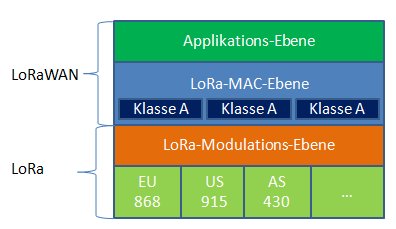
\includegraphics[width=\textwidth]{LoraLayer}
                \caption{LoRaStack \cite[S.7]{WhatIsLoRa}}
            \end{figure}
            Das Schichtenmodell lässt sich in zwei Teile unterteilen. Der LoRa Teil ist der unterste und kümmert sich 
            um die physikalische Übertragung der Pakte und er LoRaWAN Teil des Modells ist für die Steuerung des 
            Netzwerkes, Implementierung der LoRaWAN-Klassen und das überprüfen / verschlüsseln der Daten zuständig.

            Die unterste Schicht des LoRa Teils ist für die Anwendung der Richtigen Frequenzen zuständig. In Europa 
            muss das ISM-Band 868 verwendet werden in den Vereinigten Staaten wird das Band 915 
            verwendet.\cite[S.7]{WhatIsLoRa}

            Die darüber liegende Schicht heißt LoRa Modulation und kümmert sich darum dass die Pakete so in die 
            Frequenz "moduliert" werden, dass der Empfänger diese korrekt und effizient empfangen und wiederherstellen 
            kann. Mehre dazu im Kapitel \nameref{sec:Modulation}

            Über der LoRa Modulation Schicht liegt die erste LoRaWan Schicht, LoRa MAC. AC steht für ``Media Access 
            Protokoll''. Dieses Protokoll wird verwendet um das Loranetz zu steuern und wie der Name schon sagt, 
            Daten zu übertragen . Diese Schicht ist außerdem für die Implementierung der einzelnen Endgeräteklassen 
            und für das Übertragen der Steuerungskommandos zuständig. Mehr zu den Klassen kann im Kapitel \
            nameref{sec:klassen} und im Kapitel \nameref{sec:protokoll} gelesen werden.

            Die oberste Schicht nennt sich Applikationsschicht und ist dafür zuständig die Nutzdaten einer Nachricht 
            passend zu verpacken, zu verschlüsseln und zu authentifizieren.
        \subsection{Netzwerkbeitritt}
            End-Geräte sind immer bestimmten Netzwerken zugeordnet. Es gibt zwei wege um ein neue End-geräte zu einem 
            bestehenden Netzwerk hinzuzufügen.
            \subsubsection{OTAA} \label{sec:OTAA}
                Die sicherste aber auch aufwendigste Methode um ein End-Gerät mit einem Netzwerk zu verbinden heißt 
                OTAA ``Over-the-Air Activation''. Hierbei muss jedes Mal wenn einem Netzwerk beigetreten werden soll 
                die Join-Prozedur ausgeführt werden. Hierfür müssen folgende 4 Konstanten Vorgegeben werden. DevEUI, 
                JionEUI , NwkKey, AppKey. \marginpar{erklären der schlüssel?}

                Näheres zu dem DevEUI und JoinEUI kann im Kapitel \nameref{sec:endgerät} gefunden werden.

                Der NWKSKEY ist für die Verschlüsslung der Datenpakete bis zu Gateway zuständig. Auch dieser Key wird 
                vom Netzwerkserver erzeugt und muss manuell in den Code eingetragen werden.\cite[S.3]{LoRaSecur}
            
                Der letzt Wert heißt APPSKEY und sichert die Kommunikation vom End-Gerät zu dem Applikationsserver ab. 
                Der Schlüssel wird genau wie der NWKSKEY vom Netzwerkserver erzeugt und verwaltet.\cite[S.3]{LoRaSecur}

                Als erstes muss das End-Gerät eine Join- oder Rejoin-Nachricht senden. Die Nachricht besteht aus der 
                JoinEUI, dem DevEUI und einer DevNonce. Mit der DevNonce sollen Replayattack verhindert werden. Diese 
                Nonce ist das beim ersten Join-Request 0 und sollte sich bei jedem Join-Request erhöhen. Unter anderem 
                deswegen muss sie auch dann noch gespeichert werden wenn kein Strom zur Verfügung steht um die Nonce 
                nicht nach jedem ausschalten zurückzusetzen. Falls von dem gleichen Endgerät eine Join-Request mit einer 
                zu kleinen DevNonce gesendet wir, wird die Nachricht ignoriert und es ist nicht möglich dem Netzwerk 
                beizutreten.

                Die Accept Nachricht besteht aus einer JoinNonce, einem NetzwerkID Net\_ID, einer Geräteadresse DevAddr,
                einem Einstellungsfeld DLSettings , einer Zeitangabe wie lange zukünftig auf eine Antwort nach dem
                senden gewartet werden muss, hier RxDelay und einer optionalen Liste an Netzwerkparameter CFList.

                Die JoinNonce wir verwendet um Replayatacken zu verhindern und muss größer sein als die zuletzt 
                gesendete um von dem Endgerät verarbeitend zu werden. Außerdem wir die Nonce benutz um Schlüssel wie 
                AppSKey herzuleiten. Für jedes Endgerät wird eine eigene Join Nonce geführt, sie sollte sich nicht 
                wiederholen. Jedes Endgerät merkt sich die letzte JoinNonce und tritt auch nur bei wenn diese großer 
                ist als die letzte empfangene.

                Die Join-Accept Nachricht wird vom Endgerät nach JOIN\_ACCEPT\_DELAY1 oder JOIN\_ACCEPT\_DELAY2 nach 
                dem Senden des Request erwarted. Sollte die Join-Accept Nachricht zu einem andern Zeitpunkt gesendet 
                werden, wird diese nicht empfangen, da das Endgerät nicht empfangsbereit ist.

                Mehr Informationen zu den Ableitungen der Schlüssel finden Sie in dem Kapitel \nameref{sec:Sicherheit}.
                \marginpar{erklären}


            \subsubsection{ABP}
                Die einfachste Art des Beitritts heißt ABP was für ``Activation by Personalization'' zu Deutsch 
                ``Aktivierung durch Personalisierung'' steht. Hierbei muss lediglich vor Inbetriebnahme des 
                End-Gerätes 3 Konstanten definiert Werden. Manche Hersteller "brennen" diese drei Werte fest in den 
                Chip ein, sodass er nicht geändert werden kann. Falls es nicht möglich ist dem Hersteller die 
                gewünschten werte zukommen zu lasse, sind solche End-Geräte nur schlecht bis gar nicht für den Beitritt 
                mittels ABP geeignet.

                Als erstes muss die DevAdr(Geräteadresse) angegeben werden. Diese Adresse existiert nur einmal im 
                Netzwerk und wird verwendet um das Endgerät zu identifizieren. Die Adresse wird vom Netzwerkserver 
                erzeugt und muss Manuel von dort kopiert werden. 

                Mit Hilfe dieser 3 Werte kann die Join-Prozedur übersprungen werden. Daher kann 
                das Endgerät direkt einem LoRa-Netz beitreten wenn es angeschaltet wird und muss nicht erst alle 
                Schlüssel neu ableiten und aushandeln. Allerdings ist diese Methode deswegen weniger sicher, da immer 
                dieselben Schlüssel verwendet werden.

                Nach Beitritt muss das ResetInd Mac Kommando im FOpt Feld gesendet werden gesendet werden solange bis 
                ein ResetConf Kommando erhalten wird. Nun ist das Gerät im Netzwerk und kann unter der eingestellten 
                Adresse und mit dem eigestellten Schlüssel arbeiten.\cite[S. 64]{LoRaSpec}    
        \subsection{Protokoll} \label{sec:protokoll}
            Das LoRaWAN Protokoll ist optimiert für Batteriebetrieben Endgeräte die drahtlos kommunizieren möchten. 
            Um energieeffizent zu sein setzt LoRa hauptsächlich auf zwei Punkte. Die Modulationstechnick und eine 
            Adaptive Dtanenrate (ADR). Auch die 
            "One-Hop" architektur trät zur energieeffizenz bei. Die Art wie LoRa siganle Moduliert wird in Kapittel 
            \nameref{sec:Modulation} besprochen. \cite[S,1 f]{LoraClasses}


            Damit der Netzwerkserver das LoRa-Netzt steuern kann wurden, wurden Mac-Kommandos eingesetzt. Mit diesen 
            Kommandos lassen sich wie schon gesehen, dem Netzwerk beitreten, mit dem Endgerät kommunizieren und 
            Frequenzen, Kanäle und vieles mehr zu steuern.
            Da die Kommandos nur für den Netzwerkserver und die Endgeräte von Bedeutung sind, werden diese nicht an 
            den Applikationsserver gesendet sonder vom Netzwerkserver herausgefiltert. Im Folgenden wird näher auf 
            die MAC-Kommandos und die Paketstruktur eingegangen.
            Ein Uplink ist ein Paket dass vom Endgerät, das Bildlich gesprochen ``unter‘‘ dem Gateway sitzt, an das 
            Gateway gesendet wir. Ein Downlink ist dem entsprächet ein Paket das vom Gateway an den Server gesendet 
            wird.
            \subsubsection{MAC-Kommandos}
            \subsubsection{LoRa-Paketstruktur}
            Die Paketstruktur kommt wie beim ISO/OSI Schichtenmodel durch das ``durchlaufen‘‘ des Stacks zustande. 
            Da im Folgenden die Paketstruktur vom Groben ins Feine Betrachtend wird, werden hier als erstes die Felder
            der Modulationsschicht betrachtet.

            Jedes Pakete besteht aus grundlegend aus 2 Felder Präambel und  PHYPalyload Falls es sich um einen 
            Uplink-Paket handelt wird noch ein CRC Code hinzugefügt: Preamble, PHYPalyload, CRC. 
            In diesem Fall spricht man von einem implizit Paket oder von dem implizitem Modus. Implizit Modus bedeute 
            dass es kein Payload Header gibt, der Felderlängen oder CRC längenangebe angibt. Diese sind somit feste 
            zuvor definierte. Im expliziten Modus werden noch 2 Felder hinzugefügt, PHDR und PHDR\_CRC. Somit sieht 
            ein expliziteste Paket folgendermaßen aus:  Preamble,PHDR, PHDR\_CRC, PHYPalyload. Auch hier gilt, im Falle
             eines Uplink-Paketes wird am Ende ein CRC Feld angefügt. Somit ergibt sich folgende Paketstruktur: 
             Preamble, PHDR, PHDR\_CRC, PHYPalyload, CRC.

            Die Preamble ist dafür gedacht dem Empfänger mitzuteilen dass gleich Datengesendet werden. Deswegen wird 
            hier nur ein Signal gesendet das ohne Informationen ist, aber von dem Empfänger wahrgenommen werden kann.

            Da Teile des LoRaWAN Protokolls geschützt sind, finden sich über die PHDR und PHDR\_CRC Felder kaum 
            Informationen. Allerdings geht hervor, dass der PHDR die Länge des PHYPayloads und die Zieladresse 
            beinhalten sollte.
            Das PHDR\_CRC Feld wird benutzt um sicherzustellen dass die empfangenen Werte korket sind. Dies wird  
            mittels des CRC Verfahrens überprüft.
            
            Wie schon mehrfach erwähnt wird in Uplink-Nachrichten ein zusätzliches CRC Feld verwendet. CRC steht für 
            Cyclisch Redundanz Check und wird verwendet um die Korrektheit der Nachricht zu bestätigen. PHDR, PHDR\_CRC 
            und das CRC Feld werden automatisch vom dem Funktransceiver (Modul aus Empfänger und Sender) hinzugefügt.

            Die LoRa MAC ebene fügt nun das PHYPalyload Feld ein. PHYPalyload steht für Physikalische Payload. Es gibt 
            3 Mögliche PHYPayloads Entweder wird ein MACPaylod eingefügt, Join-Rejon-Request oder aber es werden die Join-Accept Nachricht darin transportiert. Um die Daten bzw. die MAC Kommandos richtig auswerten zu können und um die Korrektheit überprüfen zu können werden einige Headers und zusätzliche Felder benötigt. Deswegen lässt sich das Feld PHYPalyload weiter unterteilen in MHDR und MACPayload. Für den Fall das der MACPaylod eine Join-rejoin oder MACPayload Nachricht ist, wir noch ein MIC Feld hinzugefügt( MHDR, MACPayload, MIC). MIC steht für Message Integrity Code und wird verwendet um die Korrektheit der des MACPayloads und des MHDR festzustellen.

            Das MHDR Feld beschreibt wie die Daten im MACPayload Feld zu deuten sind. Wieder wird dieses Feld in 
            Unterfelder Unterteilt. MType, RFU und Major heißen die Unterfelder. Das MType Feld beschreibt die Art der 
            Nachricht. z.B: kann hier angegeben werden ob es sich um Datennachrichten, Join-Nachrichten, ... handelt. 
            RFU steht für ``Reserved for Future Usag‘‘ zu Deutsch ``für zukünftige verwendeung reservier‘‘.Daher kann 
            dieses Feld in der version 1.1 und niedriger ignoriert werden. Das Major Unterfeld wird verwendet um das 
            LoRa-Version der Nachricht zu definieren. Momentan ist nur der Wert 0 Definiert. 0 Steht für LoRaWan R1. 
            Die restlichen werde sind für zukünftige Updates reserviert.

            Mit der Unterteilung des MACPayload springen wir in dem LoRaStack noch eine ebene höher, in die 
            Applikationsschicht. Enthalten im MACPayload Feld sind der Frameheader FHDR, der Frame Port FPort und der 
            Frame Payload FRMPayload. Daten die gesendet werden sollen befinden sich in dem FRMPayload Feld. Wenn keine
            Daten gesendet werden, kann das FRMPayload Feld auch MAC-Kommandos enthalten. In dem Feld FPorts wird 
            angegeben an welchen Port und somit an welche Teilapplikation des Applikationsserver die Daten geleitet 
            werden sollen. Es gibt einige feste Ports. Port 0 ist reserviert um MAC-Kommandos im FRMPayload Feld 
            entgegenzunehmen. Die Ports 0x01 bis 0xDF sind Anwendungsspezifische Ports und Port 0xE0 ist für das 
            LoRaWAN Test Layer Protokoll reserviert. Falls ein anderer Port als die geraden genannten angegeben wird, 
            wird die Nachricht verworfen. 

            Erneut kann der FHDR "Frame Header" in einzelne Felder unterteilt werden in DevAddr, FCtrl, FCnt, Fopts. 
            In dem Feld DevAddr wird die Zieladresse der Nachricht vermerkt. Im Feld FCnt (Frame Counter) wird der 
            jeweilige counterwert für die bisher gezählten Nachrichten übermittelt. Hamit schützt man sich vor 
            Replayattacks. Mehr zu den Counter kann im Kapitel \nameref{sec:Sicherheit} gelesen werden. Im FOpt Feld 
            können bis zu 5 MAC Kommandos parallel zu Daten übermittelt werden. Die Anzahl kommt auf die Menge der 
            mitgelieferten Variablen an. 

            Das Letzte Feld das in Unterfelder unterhielt werden kann ist das FCtrl Feld. Hier wird das Verhalten des 
            Gerätes gestiert sowie Nachrichten bestätigt. Es gibt leichte unterschiede für ein Uplink und für Downlink 
            Nachrichten. Beide Nachrichtentypen haben ein ADR, ein ACK und ein FOptsLen Feld. Im ADR wird definiert 
            ob der Sendende bereit ist im Modus "Adaptive Data Rate" Daten zu senden, siehe Kapitel\nameref{sec:ADR}. 
            Mit dem ACK Feld können empfangene Nachrichten bestätigt werden. Ob Nachrichter bestätigt werden müssen 
            steht im MType Feld(Confirmed Data). In dem FOptsLen Feld wird die Länge des FOpts Feldes mitsamt des 
            Headers eingetragen Wenn Das FOptsLen 0 ist, ist kein FOpts Feld vorhanden.

            Ein Downlinkpaket hat zusätzlich ein RFU Feld das nicht verwendet wird und ein FPending Feld. In diesem 
            Feld kann das Gateway bzw. der Netzwerkserver dem Endgerät mitteilen, dass noch mehr Daten zu senden sind.

            Dahingegen hat ein Uplinkpaket ein ClassB Feld indem das Endgerät dem Gateway mitteilt, dass es gerne auf 
            Funktionsklasse B wechseln würde und ein ADRACKReq Feld. Dieses Feld wird verwendet um zu überprüfen ob 
            das Netzwerk noch antwortet. Die genaue Funktionsweise ist im Kapitel \nameref{sec:ADR} erklärt.

            Eine noch genauere Darlegung der LoRa-Paketstruktur kann in den LoRaWA 1.1 Specification \cite{LoRaSpec} 
            gefunden werden.

            \marginpar{Tabellen einfügen, belegen}
            \marginpar{maccomandos einfgen zuerset}   
            
            
        \subsection{Übertragungsart}\label{sec:Modulation}
            Um die Entstandenen Pakete in Signale umzusetzen und diese effizient und gleichzeitig übertragen zu können
            nutzt LoRa Chirp-Spread-Spectrum (CSS). Hierbei werden die Frequenz über eine gewisse Zeit hinweg 
            veränder. Durch messen in welche richtig, ansteigen oder abfalle, die Frequenz verändert wird, können 1 
            und 0 Codiert werden. Man spricht bei einem Bit von einem Chrip-Impuls. Durch aneinanderreihe der 
            verschiedenen Impulsen ist es möglich mehrere Bits nacheinander zu übertragen. Das entstandene Signal 
            wird auch al Sub-Chrip bezeichnet. Durch verwenden von Unterschiedlichen ansteigezeiten und abfallzeiten 
            ist es möglich mehre Signale auf der selben Frequenz zu übertragen ohne das die Signale sich gegenseitig 
            stören. Dies nennt man auch Spreading Factor. Außerdem kann die Parallelität durch verschiedene 
            Frequenzbereiche verbessert werden. CSS ist besonders für große Reichweiten geeignet und somit auch 
            bestens für Lora. Am besten ist das Signal wenn das Endgerät nahe am Gateway ist. Je weiter es entfernt 
            desto schlechter wird das Signal. Um die Kommunikation trozdem zu ermöglichen wird der ``Spreading 
            Factor‘‘ erhöht. Dies hat auch den Vorteil dass der Energieaufwand gering gehalten werden kann. 
            Analog wie Menschen auf einer Party nicht immer versuchen lauter sonder besonders langsam und deutlich 
            sprechen.\cite{explain}

            Diese Aufteilung durch den Spreading Factor und die Frequenz werden Channels erzeugt. Channels können 
            beliebig benutzt werde. es gibt allerdings mpssen zwei regeln zu beachtet werden: 
            \begin{enumerate}   
                \item Channels werden per Pseudozufallszahl geändert
                \item Sendezeit erfüllt die Regionalen Bestimmungen
            \end{enumerate}
            
            Das Aloha Protokoll wird verwendet um festzustellen wann gesendet werden soll. Dabei wird einfach gesendet
            wenn Daten zum Senden vorhanden sind. Wenn nun zwei Sender gleichzeitig auf dem selben Channel senden 
            möchten kommt es zu einer Kollision. Dadurch kann das Gateway die empfangenen Daten nicht mehr auswerden 
            und die Daten müssen erneut übertragen werden. Deswegen warten beide Endgeräte eine zufällige, 
            unterschiedliche Zeit ab bist sie erneut senden.
            
            \marginpar{frequenzy hopping}

            \subsubsection{Adaptive Data Rate}\label{sec:ADR}
            Adaprive Data Rate oder kurz ADR wird verwendet um immer die optimalste Senderate und die optimale 
            Sendepower für das Endgerät zu finden und so schnellstmöglich die Daten zu senden. ADR kann nur 
            verwendet werden wenn im FHDR Feld des LoRa-Paketes das ADR Bit gesetzt ist, siehe 
            \nameref{sec:protokoll}.Die Steuerung durch ADR findet durch den Netzwerkserver statt. Sobald der 
            Netzwerkserver bereit ist, setzt er das Bit im Downlink-Paket. Ist das Endgerät ebenfalls bereit 
            setzt es ebenfalls das Bit und ADR kann verwendet werden. Falls es nicht möglich sein sollte ADR zu 
            verwenden sollte es durch das Applikationsslayer gesteuert werden.

            Die Steuerung findet durch spezielle MAC-Kommandos statt. Standardgemäß wird die höchste 
            Übertragungsstärke verwendet und die geringste Übertragungsrate. Falls diese gedrosselt werde soll 
            wird vom Netzwerkserver das LinkADRReq MAC –Kommando benutzt. Mit diesem wird das Endgerät informiert, 
            dass es die Übertragungsstärke, Übertragungsrate oder den Übertragungskanal ändern soll. Die Werte sind 
            in den Parameter codiert. Sobald die Werte geändert wurden, muss periodisch überprüft werden ob das 
            Netzwerk die Nachrichten noch bekommt. Deswegen wird jedes Mal wenn der wenn ein Uplink empfangen wird, 
            wird der ADR\_ACK\_CNT Zähler erhöht. Wenn dieser Zähler ein gewissen schwellenwert (ADR\_ACK\_Limit) 
            überschreitet, wird das ADRACKReq Bit im Uplink gesetzt. Dieses signalisiert den Netzwerkserver das er 
            mit einem ein Nachricht senden muss um die Verbindung zu bestätigen. Falls dieser Downlink nicht in 
            ADR\_ACK\_Delay Frames empfangen wird, wird zuerst die Übertragungsstärke auf das Maximum gesetzt. 
            Falls möglich wird außerdem die Datenrate verringert um die Reichweite zu erhöhen. Die Datenrate wird 
            solange weiter, jede ADR\_ACK\_Delay Frames, verringert bis diese minimal ist. Falls diese schon 
            minimal ist müssen alle Kanäle benutzt werden. Dies wird solange probiert biss eine Verbindung 
            hergestellt werden kann. \cite[S.19 f]{LoRaSpec}         
    \section{Lora Geräte Klassen} \label{sec:klassen}
        Um maximal Energie zu sparen aber trotzdem die Möglichkeit dass die Endgeräte agile Daten empfangen können 
        wurden die Geräteklassen eingeführt. Das Hauptmerkmal der Klassen sind die unterschiedlichen Empfangsmodien. 
        Es gibt 3 Klassen, A, B und C. Die Klasse A muss standartgemäß von jedem Endgerät implementiert werden. B 
        und C sind Optional und müssen nicht vorhanden sein Alle Geräte die mehr als Klasse A unterstützen werden 
        als ``higher Class end-devices ‘‘ genannt. \cite[S.10]{LoRaSpec}
        \subsection{Klasse A}\label{sec:ClassA}
            Klasse A wird auch (All end-Devicec) genannt, zeichnet sich durch den geringsten Stromverbrauch aus. Die 
            Kommunikation wird von dem Endgeräte gestartet werden. Das bietet die Möglichkeit dass das Endgerät, wenn 
            keine Daten gesendet werden müssen, in einen sehr sparsamen Schlafmodus wechselt. Um das Endgeräte nicht 
            zum ``aufwachen‘‘ zwingen zu müssen, wurde auf einen Hardbeat oder ähnliches verzichtet. Dadurch kann das 
            Endgerät so lange ``schlafen‘‘ wie es möchte. Klasse A erlaubt außerdem das das Endgerät andere Protokolle 
            verwendet solange es keine LoRa Daten sendet oder empfängt. \cite[S.11 ff.]{LoRaSpec} Das Endgerät startet 
            die Kommunikation in dem es Daten an das Gateway sendet. Daraufhin hat das Gateway die Möglichkeit 2 mal 
            Daten zum Endgeräte senden. Die Empfangsfesnter werden RX1 und RX2 genannt. 

            Die Empfangsfesnter RX1 und RX2 müssen mindestens solange geöffnet bleiben das sie eine beginnende 
            Übertragung feststellen können. Falls keine Übertragung empfangen wird, wird das Empfangsfesnter wieder 
            geschlossen. Empfangsfenster RX1 wird nach RECIEV\_DELAY1 zeiteiheiten +/- 20msec nach Beendigung des 
            Uplinks geöffnet. Es wird die selbe Frequenz und Datenrate verwendet die auch bei den Downlink verwendet 
            wurde. Wenn festgestellt in RX1 festgestellt wurde das keine Weiteren Daten mehr empfangen werden müssen 
            kann auf das öffnen des RX2 Fensters auch verzichtet werden.

            RX2 wird wird nach RECIEV\_DELAY2 Zeiteinheiten +/- 20msec nach Beendigung des Uplinks geöffnet. Allerdings
            ist die Datenrate und Frequenz fest. Nur mittels spezieller MAC Kommandos kann dies verändert werden.
            
            Für die Join-Prozedur wird immer die Klasse A verwendet. Die verwendete Frequenz entspricht der 
            Empfangsfenster RX1 oder RX2.
        \subsection{Klasse B}
            Die Klasse B (B für BEACON) bietet bidirektionale Kommunikation mit einer deterministischem Downlink Latenz.
            Um diese Latenz zu gewährleisten, muss die Kommunikation synchronisiert ablaufen. Außerdem muss 
            festgestellt werden, ob das Endgerät bzw. das Gateway noch in Reichweite ist. Dies wird mittels eines 
            periodischem Beacon ermittelt. Dieser Beacon wird regelmäßig vom Gateway gesendet und dient der 
            Synchronisation der Endgeräte. Zeitpunkten gesendet werde realisiert. Die Latenz ist einstellbar und kann 
            bis zu 128 Sekunden.\cite[S.66 ff.]{LoRaSpec}

            Die Endgeräte öffnen in regelmäßigen Abständen ein Empfangsfenster das Pingslot genannt wird. Ein Downlink 
            der in einem Pingslot gesendet wird, wird Ping genannt. Da immer das Gateway mit dem besten empfang die 
            Daten an das Gateway sendet, muss das Endgerät selbständig feststellen wenn es einen Beacon mit einer 
            unbekannten ID bekommt und durch eine Uplink dem Server mitteilen das es sich in einer neuen Umgebung ist. 
            Dadurch lernt der Server wo sich das Endgerät befindet und kann das Gateway mit dem besten Empfang wählen.
            Obwohl das Endgerät durch die periodischen Beacon nicht ``schalfe‘‘ kann, ist die Klasse B für den 
            Batteriebetrieb gedacht.

            \subsubsection{Klassenwechsel A nach B}
                Um einen Wechsel überhaupt zu ermöglichen muss der Netzwerkserver die Standard Pingslot Periode, die 
                Pingslot Datenrate und den Pingslot Kanal kennen. Ale Endgeräte treten in Klasse A dem Netzwerk bei. 
                Das wechseln in die Klasse B wird durch folgenden Prozess realisiert.

                Als erstes muss das Programm des Endgerätes beim LoRaWAN Layer anfragen ob es möglich ist in Klasse B 
                zu wechseln. Der Layer sucht nun nach einem Beacon. Wird ein Beacon entdeckt, wird die BEACON\_LOCKED 
                Serviceprimitive \marginpar{erklären} zurückgeliefert. Wenn kein Beaconempfangen wurde wir die 
                BEACON\_NOT\_FOUND primitive zurückgegeben. Um diesen Prozess zu beschleunigen kann das DeviceTimeReq 
                MAC-Kommando verwendet werden. Damit wird das Gateway aufgefordert einen Beacon zu senden. Nun kann 
                das Endgerät in den Modus B wechseln.

                Als Zweites setzt der MAC Layer des Endgerätes das Class B Bit im FCtrl Feld des Upliks auf 1. Der MAC 
                Layer ist auch verantwortlich die Pingslot und für die Beacons Empfangsfenster zu offen. Dabei muss mit 
                der größten möglichen Abweichung der internen Uhr gerechnet werden und demensprechend die 
                Empfangsfenster angepasst werden. Diese darf pro Beacon nicht mehr als +/- 1.3msec liegen. 
                \cite[S.73]{LoRaSpec}Der Inhalt des Empfangenen Beacon wird mit der Signalsterke dem Programm des 
                Endgerätes zur weiteren Verarbeitung gesendet. Damit kann z.B. die innere Uhr nachgestellt werden 
                oder Ortswechsel festgestellt werden.
            \subsubsection{Betrieb}
                Damit der Netzwerkserver dem Endgerät mitteilen kann dass die Pingslot Frequenz und die Datenrate 
                geändert werden soll gibt es den PingSlotChannelReq Mac-Kommando. Die neuen Werte sind in den 
                Argumenten enthalten.
                        
                Das Endgerät kann die Periode der Pingslot szu einer beliebigen Zeit ändern. Ist dies der Fall, so 
                muss das Endgerät in Klasse A wechseln und mittels dem MAC-Kommando PingSlotChannelReq die geänderte 
                Periode Mitteilen. Danach kann zurück in die Klasse B gewechselt werden.

                Falls einige länger als 2 Stunden kein Beacon empfangen wird, kann die Synchronisation mit dem Netzwerk 
                verloren gehen. Dadurch funktioniert die Kommunikation in Klasse B nicht mehr und es wird in Klasse A 
                gewechselt. Nun kann versucht werden eine Verbindung mit der Klasse A aufzubauen. Das Programm des 
                Endgerätes kann versuchen wieder in Klasse B zu wechseln. Dieser Prozess kann sich immer wieder 
                wiederholen.

                Um auch innerhalb der minimal 2 Standen in den kein Beacon empfangen wurde einen Kommunikation zu 
                ermöglichen wird jedes Mal wenn ein Beacon verloren geht in den Beacon-Less Modus gewechselt. Dieser 
                Modus orientiert sich ausschließlich an der internen Uhr.
                Um die Abweichung auszugleichen werden die Empfangsfenster immer früher begonnen und immer später 
                beendet. Das bedeutet einen höheren Energieverbrauch aber auch eine höhere Wahrscheinlichkeit noch 
                Daten zu empfangen obwohl die Uhren des Gateways und des Endgerätes auseinanderlaufen.

            \subsubsection{Singel / Multicast}
                In Klasse B können die Nachrichten als Singelcast oder als Multicast Nachrichten verwendet werden. 
                Eine Singelcast Nachricht wird an des Endgerät das im DevAfdr Feld der Nachricht codiert ist gesendet.
                Im Multicastmodus wird das Paket an mehrere Endgeräte gesendet. Damit dise möglich ist müssen sich 
                die Endgeräte dieselbe Multicast Adresse und die dazugehörigen Schlüssel teilen. Durch verschiedene 
                Multicastadresse ist es möglich sogenannte Multicastgruppen zu erzeugen die nicht alle sonder nur ein 
                Teil aller Endgeräte beinhalten. LoRaWAN gibt allerding keine Methode vor wie die Adressen und 
                Schlüssel verteilt werden. Diese Aufgabe muss in der Applikationsebene sprich im Programm der 
                Endgeräte bzw. des Applikationsserver oder die Schlüssel und Adresse werden fest in den Programmcode 
                programmiert.

                In Multicastnachrichten sind keine MAC-Kommandos erlaubt. Nur Daten dürfen als Multicastnachrichten 
                übertragen werden. Dies wurde eingeführt da Multicastnachrichten nicht dieselbe Robustheit wie 
                Singelcastnachrichten haben. Die Nachrichten dürfen nicht bestätigt werden da sonst eine große Last 
                für das Netzt entstehen würde.\cite[S.84]{LoRaSpec}

            \subsubsection{Beacon}
                Wie schon erwähnt werden der Beacons verwendet um das Endgerät mit dem Netzwerk zu synchronisieren. 
                Deswegen werden die Beacon Periodisch gesendet. Die Zeit zwischen zwei Beacon wir BEACKON\_Period 
                genannt. Die Endgeräte öffnen Empfangsfenster um diese Beacons zu empfangen. Ein Beacon zu übertragen 
                dauert BEACON\_RESERVED lange. Das Beacon-Empfangsfenster wird BEACKON \_GUARD früher geöffnet um 
                sicher zu stellen das Beacon auch wirklich erkannt werden kann. Außerdem wird die Beakon\_GUARD 
                benutzt um sicherzustellen dass kein Pingslot mehr geöffnet ist. Deswegen muss diese Beakon\_GUARD 
                mindestens so lang sein wie ein maximaler Pingslot. Das hat den Vorteil, dass nicht darauf gedacht 
                werden muss wann ein Pingslot geöffnet wurde, da er im Zweifelsfall fertig ist bevor ein Beacon 
                empfangen wird. Vergleichbar ist dies mit der Distributed Coordination die bei WLAN Anwendung findet.

                Während versucht wird ein Beacon zu empfangen kann kein Pingslot geöffnet werden
                
                Um Synchronisierungen durch die Beacon zu vermeiden, wie ``alle Endgeräte wollen sofort nach den 
                Beacon senden wollen‘‘, wird mittels zufälliger Wartezeiten und zufälliger Pingslotperiode verhindert. 
                Durch den Zufall wird die Wahrscheinlichkeit deiner Kollision geringer.

                Beacons haben ihr eigenes Paketformat. Diese Pakete sind immer gleich lang. Dadurch kann auf Header 
                verzichtet werden was auch der Verarbeitungsgeschwindigkeit zugutekommt. Wie auch ein normales 
                LoRa-Paket, so besteht auch das erste Feld des Beacon-Paketes aus der Preable. Danach folgt der 
                BCNPayload. Der BCNPayload(Beacon Payload) lässt sich unterteilen in RFU, Time, CRC, GWSpecific, 
                RFU, CRC. Die zwei CRC Felder weisen schon auf die logische Unterteilung in zwei hältern hin. Der 
                erste Teil enthält Beacon spezifische Informationen (time und CRC). In dem Time Feld ist die Zeit 
                seit 00:00:00, 01.01.1980 Modulo 2\^32 enthalten. das CRC Feld wird verwendet um die Korrektheit des 
                Zeit und des RFU Feldes zu versichern. RFU steht wieder für ``Reserved for Future Usage‘‘ und wird 
                nicht verwendet. Die andere Hälfte ist Gatewayspezifisch. Sie enthält das GwSpecific Feld und ein 
                RFU Feld . Beide Fleder sind  durch ein zweites CRC Feld abgesichert ist. Das GwSpezific Feld lässt 
                sich unterteilen in InfoDesc und Info Felder. Das InfoDesc gibt an auf was sich das Infofeld bezieht. 
                0 gibt an das die GPS-Koordinaten der ersten Antenne folgen. 1 steht für die GPS-Koordinaten der 
                zweiten Antenne und 2 steht für die GPS-Koordinaten der dritten Antenne. Die werte 3 bis127 sind noch 
                Solange sich im Info Feld Koordinaten enthalten kann dieses unterteilt werden in Längen- und 
                Breitengrad.
                
                Auch Klasse A kann den Beacon nutzen, um herauszufinden von welchem Gateway es gerade Datenempfängt 
                und um eventuelle Standortwechsel festzustellen.
                
                In Europa werden die Beacons auf einer festen Frequenz übertragen die sich nicht ändert. Nur über das 
                MAC-Kommando PingSlotChannelReq. 
        \subsection{Klasse C}
            C steht für CONTINUOUSLY Listening. Wie der Name schon sagt ist hier dauernd ein Empfangsfenster geöffnet.
            Dafür wird es ermöglicht fast Latzen frei zu übertragen. Dies bedeutet aber auch das der Stromverbrauch am 
            höchsten ist und somit die Klasse C nicht für den Batteriebetrieb geeignet. 

            Geräte die Klasse C implementieren sollen aus nicht die Klasse B implementieren das es sonst zu fejlern 
            kommen kann.

            Diese Klasse verwendet die Gleichen Empfangsfenster mit der gleichen Frequenz wie in Klasse A. Der große 
            unterscheid besteht allerdings darin das RX2 immer dann geöffnet ist wenn nicht gerade Daten an das 
            Gateway gesendet werden oder RX1 geöffnet ist. 

            Auch in Klasse C ist es, wie in B, möglich Multicastnachrichten zu senden. Hierbei gelten die gleichen 
            Regeln wie bei Klasse B.

    \section{Sicherheit} \label{sec:Sicherheit}
    Jede Klasse hat 3 Zähler: FCntUP(wird für jeden Uplink erhöh), NFCntDown (pro downlink für MAC-Kommandos), AFCntDOwn(Downlinks die Daten enthalten) Zähler sollen nich flüchtig sein(Batteriewechseln kein reset) bei neuverbinden müssen alle counter auf uf 0 gesetzt werden. counter müssen auf beiden seiten glich gehalten werden(Synchron geführt) nachricht empfagen ist muss der darin enthaltenene counter größer sein als der eigene. 

    die Counter Werte sollen so weit wie möglich nur einam verwendet werden.
    
    )
    \


        \marginpar{Weche felder was ist wie verschlüsselt?}
                
        SIcherheit in netzwerkfägigen Systemen ist ein sher wichtiges und heiß dikutiertes thema. Da LoRa daten Üver die Lpft überträgt, ist es extrem wichtig sich und die Dtaen zu schützen.
        Da Luft als Medium benutzt wird könnten alle in der Nähe befindlichen geräte die gesendeten Daten mithören. Aber genauso kann ein Endgerät sich als ein andres ausgeben und in seinem Namen Daten an ein
        Fremden Server send. Um zu verhindern das Gesnedene Daten mitgelsen werden müssen diese verschlüsselt werde. Um zu verhindern das jemand anderst so tut als wäre er das engerät mussen die Dtane Autentifiziert werden.
        Slest jetz könnten z.B. Join-request mitgeschnitten werden und von dem (bößen) endgerät wiederholt werden um das (gut) endgerät daran zu hindern aktiv dem Netzwerk beizutreten. Deswegen wurden zähler eingebaut. Im folgenden wird sich nächer damit beschäftigt welche mechanismen es gibt die gennten probleme zu umgehen.
        
        Oberflächlich gesehen bietet Lora eine end-to-end Sicherheit an, indem es die Signale zweimal verschlüsselt.
        Die erste Verschlüsselung dient dazu die gesendeten Daten vor eventuellen Mithörern zu verschlüsseln, also pm Endgerät bis zu Gateway zu verschlüsslen. Die Verschlüsselung geschieht mit einem 128-bit Network-Session-Key.
        Die zweite Verschlüsselung wird bis zur endgültigen Weiterverarbeitung der Daten auf z.B. einen Server verwendet und ist ein 128 bit Application-Session-Key.

        Nächer betrachtd benutzt Lore eine ganze Reihe an Schlüssel und Zähler verwendet um die Kommunikation abzusichern. Da die verwendeten Schlüssel bei OTAA-Aktivation variieren wird hier eine viel höhere Sicherit geboten als bei ABP-Activation wo alle Schlüssel von anfangan vorgegeben werden.
        Infolgedessen wird im folgenden Text auf die SIcherheit unter verwendung von OTAA bezogen.

        Jesed enggerät hat seine eigenen NwkKey (Netzwerkschlüssel) und AppKey (applikation schlüssel). Sobald einem Netzwerk begetreten wurde wird aus dem NwkKeay der FNwkSIntKey , SNwkSIntKey und NwkSEncKey
        abgeleited. AUs dem AppKey iwrd zusätzlich der AppSKey abgeleited. Die schlüssel müssen so gespeichert werden, dass es nicht mölgich ist diese auf irgendeiener weise aus dem Speicher zu holen außer für das endgerät selber.
        Zusätzlich werden Join-Keys abgeleited. JSInitKEy und JSEncKey.

        Der FNwkSIntKey ist einzigartig für ein Endgerät und heist Forwarding Network session integrity key. Der Schlüssel wird verwendet um ganze oder Teile der MIC felder in den LoRapaketen zu berechen \marginpar{mic}. 
        
        Serving Network session integrity key heißt abgekützt SNwkSIntKey. Dieser Schlüssel wird
        verwedent um die Integrität des MIC codes zu überprüfen. Zusätzlich wird er auch verwendet um Teile des MIC codes zu berechen. Dieser Schlüssel ist spezifisch für ein entgerät.
        
        NwkSEncKey oder lang Network session encryption key, ist für jede Netzwerksitzung einzigartig und wurd verwendet um empfnagen order gesendete
        Mac kommandos zu ent- oder verschlüsseln.
        
        Der AppSKey wird auch Application session key und wird einem Endgerät zugeordent. Er wird vom Gateway und vom Endgerät verwendet um  Daten die zum Applikationsserver geschickt werden sollen zu verschlüsseln.
       
        pad fügt do viele 0en das die länge an vielfaches von 16 ist
        AppSKey = aes128\_encrypt(NwkKey, 0x02 | JoinNonce | NetID | DevNonce | pad16) 
        FNwkSIntKey = aes128\_encrypt(NwkKey, 0x01 | JoinNonce | NetID | DevNonce | pad16)
        SNwkSIntKey = NwkSEncKey = FNwkSIntKey.

        \bigbreak

        Jedes Gerät hat 3 verscheidene Frame counter um die Anzahl der gesendeten und empfangenen Frams mitzuzählen der FCntUP counter zählt die
        uplikframes, der NFCNTDown zählt die MAC-downlinkframes und der AFCntDown welcher alle downlinkframes zählt die Nutzdaen enthalten.

        Wenn ein gerät dem Netzwerk beitritt, werden zuerst die Counter auf 0 gesetzt. Beide seiten einer Kommunikation halten die zähler gleich. 
        Beim senden wird der Aktulle counterwert in das FCnt feld eingetragen. Werden übertragungen wiederholt so wird der counter nicht erhöht \marginpar{weiderholung schon drin?}

        Durch das verwerfen von NAchrichten mit zu kleinem Counterwert, wird verhindert das Pakete von einem Angreifer aufgenommen und zu einem späteren Zeitpunkt wiederabgespielt werden.
        
        Jauch bei den Join oder Accept NAchrichten besteht die gefahr eine Replayattac. Da hier dem Netzwerk noch nicht begetreten wurde, können die zähler niht verwendet werden. Hier wird eine Nonce in die 
        Join-Pakete coderit \marginpar{wie sieht paket aus.}. DIese Nonce zählt auf die gleiche weise hoch wie die counter. Die gegnerische Seiter der Kommunkikation muss die Nonce tracken und darf nur pakete mint einer Nonce akzeptieren die höher ist als die letzt Nonce.\marginpar{frequncyhopping}
       
        \cite{LoRaSecur}(Netzwerkserver hat AppKey daraus werden AppSKeay und NwkSkey erzeugt)
        \cite{WhatIsLoRa}(Applikationsverschlüsselung(schutz der Daten for mitlesen) Netzwerk(Autentiizierung der Knoten) AFS, Key Exnage IEEE EU164)
        \cite{LoRaSpec}(symetrischer Schlüssel => nur einer benötigt, Sessionkey ist abgeleited von Knoten-rootkey. JoinServer setllt verbindung der Keys her.
        )
    \section{Live-Beispiel}
        wenn vorhanden.

    \section{Ausblick}

    Sobald dem Netzwerk erfolreich beigetreten wurde werden ein die benötigten schlüssel aud dem vorher gesetzetn Werten abgeleited. genauers dazu in kapitel \nameref{sec:Sicherheit}.
    \marginpar{unconfirmed / confirmed, regionale Parameter}.
    %\section{Sonstige quellen}
    %    \url{https://lora-alliance.org/resource-hub}
    %    QuickStart für ein kleines Projekt: \url{https://www.thethingsnetwork.org/docs/devices/node/quick-start.html#setup-arduino-ide}
    %  
    %   Weitere Infos \url{http://www.multitech.com/documents/publications/marketing-guides/lora_device_dev_guide_orange.pdf}
        \newpage
    \bibliographystyle{geralpha}
    \bibliography{myBib}
    %richtige namen finden
\end{document}